\documentclass[12pt,a4paper]{report}

% ---- Encodage ----
\usepackage[utf8]{inputenc}
\usepackage[T1]{fontenc}

% ---- Mise en page ----
\usepackage[top=2.5cm, bottom=2.5cm, left=3cm, right=2.5cm]{geometry}
\usepackage{fancyhdr}
\usepackage{emptypage}
\usepackage{setspace}
\usepackage{parskip}

% ---- Couleurs ----
\usepackage{xcolor}
\definecolor{enspyorange}{RGB}{220,110,0}
\definecolor{enspyblue}{RGB}{0,60,130}
\definecolor{darkblue}{RGB}{0,40,100}
\definecolor{lightblue}{RGB}{235,243,255}
\definecolor{codegreen}{RGB}{30,140,30}
\definecolor{codegray}{RGB}{120,120,120}
\definecolor{codeblue}{RGB}{0,90,190}
\definecolor{codebg}{RGB}{250,250,254}
\definecolor{darkgray}{RGB}{70,70,70}
\definecolor{rowgray}{RGB}{245,245,245}

% ---- Graphiques ----
\usepackage{graphicx}
\usepackage{float}
\usepackage{subcaption}
\usepackage{tikz}
\usetikzlibrary{shapes,arrows.meta,positioning,calc,decorations.pathreplacing}

% ---- Tableaux ----
\usepackage{booktabs}
\usepackage{tabularx}
\usepackage{multirow}
\usepackage{array}
\usepackage{colortbl}
\usepackage{longtable}

% ---- Code ----
\usepackage{listings}
\lstset{
  backgroundcolor=\color{codebg},
  basicstyle=\ttfamily\small,
  breaklines=true,
  captionpos=b,
  commentstyle=\color{codegreen}\itshape,
  frame=single,
  frameround=tttt,
  keywordstyle=\color{codeblue}\bfseries,
  language=Python,
  numbers=left,
  numbersep=8pt,
  numberstyle=\tiny\color{codegray},
  rulecolor=\color{codegray!40},
  showstringspaces=false,
  stringstyle=\color{enspyorange},
  tabsize=4,
  xleftmargin=15pt,
  morekeywords={import,from,as,def,class,return,True,False,None,
                torch,nn,np,self,super}
}
\lstdefinestyle{bash}{
  language=bash,
  backgroundcolor=\color{darkblue!7},
  basicstyle=\ttfamily\small\color{darkblue},
  keywordstyle=\color{enspyorange}\bfseries,
  frame=single,frameround=tttt,
  rulecolor=\color{darkblue!30},
  numbers=none,breaklines=true,
}

% ---- Boites ----
\usepackage{tcolorbox}
\tcbuselibrary{skins,breakable}

\newtcolorbox{cmdbox}[1][]{
  enhanced,breakable,
  colback=darkblue!6,colframe=darkblue!50,
  fonttitle=\bfseries\small\color{white},
  colbacktitle=darkblue,
  title={Commande PowerShell},
  arc=4pt,boxrule=0.8pt,left=4pt,right=4pt
}
\newtcolorbox{infobox}[1][Information]{
  enhanced,breakable,
  colback=lightblue,colframe=enspyblue,
  fonttitle=\bfseries\small\color{white},
  colbacktitle=enspyblue,
  title={#1},arc=4pt,boxrule=0.8pt
}
\newtcolorbox{resultbox}[1][Resultats]{
  enhanced,breakable,
  colback=green!5,colframe=codegreen!70,
  fonttitle=\bfseries\small\color{white},
  colbacktitle=codegreen!80,
  title={#1},arc=4pt,boxrule=0.8pt
}
\newtcolorbox{warningbox}[1][Attention]{
  enhanced,breakable,
  colback=enspyorange!8,colframe=enspyorange,
  fonttitle=\bfseries\small\color{white},
  colbacktitle=enspyorange,
  title={#1},arc=4pt,boxrule=0.8pt
}
\newtcolorbox{arbobox}[1][Arborescence]{
  enhanced,breakable,
  colback=codebg,colframe=codegray!50,
  fonttitle=\bfseries\small\color{white},
  colbacktitle=darkgray,
  title={#1},arc=4pt,boxrule=0.8pt,
  left=4pt,right=4pt,
  fontupper=\ttfamily\small
}

% ---- Maths ----
\usepackage{amsmath}
\usepackage{amssymb}

% ---- Liens ----
\usepackage{hyperref}
\hypersetup{
  colorlinks=true,
  linkcolor=enspyblue,
  urlcolor=enspyorange,
  citecolor=darkblue,
  pdftitle={Rapport Projet 1 - LightGCN - BILOA ABADJECK Paolo},
  pdfauthor={BILOA ABADJECK Valery Paolo Stelane}
}

% ---- Divers ----
\usepackage{enumitem}
\usepackage{pifont}

% ---- Titres de chapitres ----
\usepackage{titlesec}
\titleformat{\chapter}[display]
  {\normalfont\huge\bfseries\color{enspyblue}}
  {\tikz[baseline]{
     \node[fill=enspyblue,text=white,minimum width=1.1cm,
           minimum height=1.1cm,rounded corners=4pt,
           font=\Large\bfseries]{\thechapter};}
  }{10pt}{\Huge}
  [\vspace{2pt}{\color{enspyorange}\hrule height 2pt}]

\titleformat{\section}
  {\normalfont\Large\bfseries\color{enspyblue}}
  {\thesection}{1em}{}
  [\vspace{-4pt}{\color{enspyblue!40}\hrule height 0.5pt}]

\titleformat{\subsection}
  {\normalfont\large\bfseries\color{darkblue}}
  {\thesubsection}{1em}{}

\titleformat{\subsubsection}
  {\normalfont\normalsize\bfseries\color{darkgray}}
  {\thesubsubsection}{1em}{}

% ---- En-tetes ----
\pagestyle{fancy}
\fancyhf{}
\fancyhead[L]{\small\color{enspyblue}\textbf{ANI-IA 4 -- ENSPY Yaounde}}
\fancyhead[C]{\small\color{darkgray}Projet 1 -- Systeme de Recommandation LightGCN}
\fancyhead[R]{\small\color{enspyblue}\textbf{BILOA ABADJECK P.}}
\fancyfoot[C]{\small\thepage}
\fancyfoot[R]{\small\color{codegray}2025/2026}
\renewcommand{\headrulewidth}{1.2pt}
\renewcommand{\headrule}{%
  \hbox to\headwidth{\color{enspyblue}\leaders\hrule height\headrulewidth\hfill}}
\renewcommand{\footrulewidth}{0.4pt}

% ============================================================
\begin{document}
\setstretch{1.25}

% ============================================================
% PAGE DE GARDE
% ============================================================
\begin{titlepage}
\thispagestyle{empty}
\begin{center}

\noindent\textcolor{enspyblue}{\rule{\textwidth}{0.55cm}}\\[-2pt]
\noindent\textcolor{enspyorange}{\rule{\textwidth}{0.18cm}}

\vspace{0.5cm}

{\color{enspyblue}\Large\textsc{Ecole Nationale Superieure Polytechnique de Yaounde}}\\[3pt]
{\color{enspyorange}\normalsize Departement du Genie Informatique}\\[3pt]
{\color{darkgray}\small
  Unite d'Enseignement : \textbf{Intelligence Artificielle et Applications -- ANI-IA 4}}

\vspace{0.8cm}

\includegraphics[width=4.8cm]{logo.jpg}

\vspace{0.7cm}

\begin{tcolorbox}[
  enhanced,colback=enspyblue!7,colframe=enspyblue,
  arc=8pt,boxrule=2pt,width=0.9\textwidth]
\begin{center}
  {\huge\bfseries\color{enspyblue} Rapport de Projet}\\[8pt]
  {\Large\color{darkgray} Systemes de Recommandation par}\\[4pt]
  {\LARGE\bfseries\color{enspyblue} Reseaux de Neurones sur Graphes}\\[6pt]
  {\large\bfseries\color{enspyorange}
    LightGCN -- Light Graph Convolutional Network}
\end{center}
\end{tcolorbox}

\vspace{0.5cm}
{\large\itshape\color{darkgray}
  Rapport de Projet $\cdot$
  Dans le cadre du cours Intelligence Artificielle et Applications}

\vspace{0.8cm}

\begin{minipage}[t]{0.46\textwidth}
\raggedright
\begin{tcolorbox}[colback=lightblue,colframe=enspyblue,arc=6pt,boxrule=1.5pt]
  {\small\bfseries\color{enspyblue} Presente par :}\\[5pt]
  {\normalsize\bfseries BILOA ABADJECK}\\
  {\normalsize Valery Paolo Stelane}\\[3pt]
  {\small\color{darkgray} Matricule : \textbf{22P009}}\\
  {\small\color{darkgray} Classe : \textbf{ANI-IA 4}}
\end{tcolorbox}
\end{minipage}
\hfill
\begin{minipage}[t]{0.46\textwidth}
\raggedleft
\begin{tcolorbox}[colback=enspyorange!10,colframe=enspyorange,arc=6pt,boxrule=1.5pt]
  {\small\bfseries\color{enspyorange} Encadre par :}\\[5pt]
  {\normalsize\bfseries M. OMGBA BITHA Junior}\\[3pt]
  {\small\color{darkgray} Module :}\\
  {\small\bfseries Intelligence Artificielle}\\
  {\small\bfseries et Applications}
\end{tcolorbox}
\end{minipage}

\vspace{0.6cm}

{\small\color{darkgray}
  \textbf{Repository GitHub :}
  \url{https://github.com/paolo-88-hub/projet1-lightgcn-AIA-4}}

\vfill

\noindent\textcolor{enspyorange}{\rule{\textwidth}{0.18cm}}\\[-2pt]
\noindent\textcolor{enspyblue}{\rule{\textwidth}{0.45cm}}\\[4pt]
{\color{white}x}\\[-14pt]
{\color{darkgray}\normalsize
  Ecole Nationale Superieure Polytechnique de Yaounde
  \quad|\quad Annee academique 2025/2026}

\end{center}
\end{titlepage}

% ============================================================
% RESUME
% ============================================================
\chapter*{Resume}
\addcontentsline{toc}{chapter}{Resume}
\thispagestyle{fancy}

Ce rapport presente la conception, l'implementation et l'evaluation d'un
\textbf{systeme de recommandation de films} base sur le modele
\textbf{LightGCN} (Light Graph Convolutional Network), realise dans le
cadre de l'Unite d'Enseignement \textit{Intelligence Artificielle et
Applications} (ANI-IA 4) a l'Ecole Nationale Superieure Polytechnique
de Yaounde.

Le projet exploite le dataset \textbf{MovieLens ml-latest-small}
(100\,836 interactions brutes, 610 utilisateurs, 3\,650 films).
Apres filtrage, 89\,664 interactions sont conservees pour
l'entrainement. LightGCN modelise les interactions sous forme d'un
\textbf{graphe biparti normalise} et propage les embeddings sur
\textbf{K=3 couches} pour capturer les collaborations de haut ordre.
L'optimisation est realisee par la \textbf{perte BPR} (Bayesian
Personalized Ranking) via l'optimiseur Adam sur 100 epoques.

Les resultats obtenus sont :
\textbf{Recall@10 = 0,0754} et \textbf{NDCG@10 = 0,0308},
avec une convergence de la perte BPR de 0,676 a 0,150 (--78\%).

Au-dela des livrables initialement remis, une
\textbf{contribution personnelle supplementaire} a ete
developpee apres reflexion : un \textbf{dashboard interactif
temps reel} (Flask + SocketIO) permettant de visualiser
l'ensemble du pipeline en direct depuis le navigateur,
avec courbes de convergence, metriques live et conclusion
automatique. Cette interface n'etait pas demandee dans les
livrables du projet initial -- elle constitue une innovation
ajoutee pour rendre le travail plus explicite et demonstrable.

\bigskip
\noindent\textbf{Mots-cles :} LightGCN, Graph Convolutional Network,
Systeme de recommandation, Filtrage collaboratif, BPR Loss,
Embeddings, MovieLens, PyTorch, Dashboard temps reel, Flask-SocketIO.

% ============================================================
% TABLES
% ============================================================
\tableofcontents
\listoffigures
\listoftables
\newpage

% ============================================================
% CHAPITRE 1 — INTRODUCTION
% ============================================================
\chapter{Introduction}

\section{Contexte}

Les systemes de recommandation constituent aujourd'hui un pilier
fondamental des plateformes numeriques mondiales. De Netflix a Spotify,
la capacite a proposer du contenu personnalise repose sur des
algorithmes d'intelligence artificielle capables d'exploiter les
interactions passees pour predire les preferences futures.

Le defi central est le \textit{filtrage collaboratif} : comment
inferer qu'un utilisateur aimera un article qu'il n'a jamais vu, en
s'appuyant uniquement sur les interactions historiques d'une
communaute ? Les approches classiques (factorisation de matrices) ont
montre leurs limites face aux donnees eparses et aux relations
complexes de haut ordre.

\textbf{LightGCN} (He et al., 2020) repond a ces limitations en
modelisant explicitement la structure du graphe d'interactions, avec
une propagation pure et elegante ne necessitant aucune transformation
ni activation non lineaire.

\section{Objectifs du projet}

\begin{enumerate}[label=\textbf{\arabic*.}]
  \item Comprendre les fondements theoriques des Graph Convolutional
    Networks et leur simplification via LightGCN.
  \item Implementer LightGCN \textit{from scratch} en PyTorch sans
    librairie tierce dediee aux graphes.
  \item Entrainer le modele sur MovieLens avec la perte BPR et
    l'optimiseur Adam.
  \item Evaluer les performances avec Recall@10 et NDCG@10.
  \item Deployer un \textbf{dashboard interactif temps reel}
    (Flask + SocketIO) montrant le pipeline en direct.
  \item Generer des recommandations Top-10 personnalisees.
\end{enumerate}

\section{Organisation du rapport}

Ce rapport suit la structure suivante : Chapitre 2 --- Etat de l'art.
Chapitre 3 --- Methodologie et environnement. Chapitre 4 ---
Implementation. Chapitre 5 --- Mode d'emploi complet. Chapitre 6 ---
Resultats et interfaces. Chapitre 7 --- Difficultes et solutions.
Chapitre 8 --- Conclusion.

% ============================================================
% CHAPITRE 2 — ÉTAT DE L'ART
% ============================================================
\chapter{Etat de l'Art}

\section{Systemes de recommandation}

Les systemes de recommandation se divisent en trois familles
principales :

\begin{description}
  \item[Filtrage base sur le contenu] Recommande des items similaires
    a ceux deja apprecies, en exploitant leurs caracteristiques
    intrinseques.
  \item[Filtrage collaboratif] Exploite les interactions collectives
    pour trouver des utilisateurs similaires. C'est l'approche de
    LightGCN.
  \item[Approches hybrides] Combinent les deux methodes pour
    beneficier de leurs avantages respectifs.
\end{description}

\section{De la factorisation de matrices aux GCN}

La factorisation de matrices (MF) fut longtemps l'etat de l'art. Elle
represente chaque utilisateur et article par un vecteur latent et
predit l'interaction par produit scalaire. Cependant, MF souffre de :
\begin{itemize}
  \item L'incapacite a capturer des relations de haut ordre.
  \item Une performance degradee sur des donnees tres eparses.
  \item L'absence de modelisation explicite de la structure du graphe.
\end{itemize}

NGCF (Wang et al., 2019) a propose de propager les informations sur
le graphe biparti utilisateur-item. Mais NGCF introduit des
transformations et activations superflues.

\section{LightGCN -- Simplification elegante}

\textbf{LightGCN} simplifie radicalement NGCF en ne conservant que
l'essentiel : la propagation pure des embeddings.

\subsection{Formulation mathematique}

Soit $\tilde{A} = D^{-1/2} A D^{-1/2}$ la matrice d'adjacence
normalisee du graphe biparti. La propagation a la couche $k$ :
\begin{equation}
  E^{(k)} = \tilde{A} \cdot E^{(k-1)}
\end{equation}

L'embedding final est la moyenne ponderee de toutes les couches :
\begin{equation}
  E^* = \frac{1}{K+1} \sum_{k=0}^{K} E^{(k)}
\end{equation}

Le score de prediction pour la paire $(u, i)$ :
\begin{equation}
  \hat{y}_{ui} = (e_u^*)^\top \cdot e_i^*
\end{equation}

\subsection{Perte BPR}

\begin{equation}
  \mathcal{L}_{\text{BPR}} = -\sum_{(u,i,j)}
  \ln \sigma(\hat{y}_{ui} - \hat{y}_{uj})
  + \lambda \|E^{(0)}\|^2
\end{equation}

ou $(u,i,j)$ est un triplet avec $i$ un item positif et $j$ negatif.

\subsection{Avantages de LightGCN}

\begin{itemize}
  \item Moins de parametres : seuls les embeddings $E^{(0)}$ sont
    appris.
  \item Interprétabilite : schema mathematique clair.
  \item Performance superieure a NGCF sur les benchmarks standards.
  \item Scalabilite grace aux matrices sparse.
\end{itemize}

\section{Dataset MovieLens}

\begin{table}[H]
\centering
\caption{Caracteristiques du dataset MovieLens ml-latest-small}
\begin{tabular}{lll}
\toprule
\textbf{Caracteristique} & \textbf{Valeur} & \textbf{Remarque} \\
\midrule
Nombre de ratings bruts & 100\,836 & Fichier ratings.csv \\
Utilisateurs & 610 & Apres filtrage \\
Films total & 9\,742 & Catalogue complet \\
Films apres filtrage & 3\,650 & Items retenus \\
Interactions train & 89\,664 & Leave-one-out \\
Interactions test & 610 & 1 par utilisateur \\
Periode & 1996--2018 & Historique long \\
\bottomrule
\end{tabular}
\end{table}

% ============================================================
% CHAPITRE 3 — MÉTHODOLOGIE
% ============================================================
\chapter{Methodologie et Environnement Technique}

\section{Environnement d'execution}

\begin{table}[H]
\centering
\caption{Methodes et Technologies Employees -- Projet 1}
\begin{tabular}{ll}
\toprule
\textbf{Composant} & \textbf{Detail} \\
\midrule
\rowcolor{lightblue!60}
\multicolumn{2}{l}{\textbf{Livrables initiaux remis}} \\
Modele & LightGCN (He et al., 2020) \\
Framework IA & PyTorch 2.12.0 + torch\_sparse (CPU) \\
Langage & Python 3.14.5 \\
Dataset & MovieLens ml-latest-small \\
Representation & Graphe biparti sparse (COO format) \\
Fonction de perte & BPR (Bayesian Personalized Ranking) \\
Optimiseur & Adam (lr=0.001) \\
Metriques & Recall@10, NDCG@10 \\
Visualisation & Matplotlib, Seaborn, t-SNE \\
Environnement initial & VS Code + PowerShell, Windows 11 \\
\midrule
\rowcolor{enspyorange!15}
\multicolumn{2}{l}{\textbf{Innovation personnelle ajoutee -- Dashboard Temps Reel}} \\
Interface web & Flask 3.x + Flask-SocketIO 5.x \\
Communication & WebSocket (protocole SocketIO) \\
Graphiques live & Chart.js 4.4 \\
Progression temps reel & Barres animees + metriques live \\
Conclusion automatique & Generee dynamiquement en fin de pipeline \\
Port & http://localhost:5000 \\
\midrule
Processeur & Intel Core i5 (CPU uniquement) \\
Repository & \url{https://github.com/paolo-88-hub/projet1-lightgcn-AIA-4} \\
\bottomrule
\end{tabular}
\end{table}

\begin{warningbox}[Note sur le GPU]
Python 3.14 n'etant pas encore supporte par PyTorch pour CUDA,
tout l'entrainement s'est deroule sur CPU Intel Core i5.
Duree totale : environ 15--20 minutes pour 100 epoques.
\end{warningbox}

\section{Livrables Attendus et Contribution Supplementaire}

\subsection{Livrables initialement prevus}

Les livrables definis dans le cadre du projet ANI-IA 4 etaient :

\begin{itemize}
  \item Code source complet et commente (Python)
  \item Graphiques de convergence (courbe de perte par epoque)
  \item Tableau de resultats Recall@10 et NDCG@10
  \item Visualisation t-SNE des embeddings
  \item Exemples de recommandations Top-10 pour plusieurs
    utilisateurs
\end{itemize}

\subsection{Contribution personnelle supplementaire -- Dashboard Temps Reel}

\begin{tcolorbox}[enhanced,breakable,
  colback=enspyorange!8,colframe=enspyorange,
  fonttitle=\bfseries\color{white},
  colbacktitle=enspyorange,arc=4pt,boxrule=1pt,
  title={Innovation personnelle -- non prevue dans les livrables initiaux}]

Apres reflexion et a l'issue du developpement du projet, j'ai
concu et implemente par \textbf{initiative propre} un
\textbf{dashboard interactif temps reel} qui ne figurait pas
dans les livrables demandes. Cette contribution supplementaire
constitue une amelioration significative de la presentation
et de la comprehension du travail realise.

\medskip
\textbf{Pourquoi ce dashboard ?} Les livrables initiaux
produisaient des resultats statiques (graphiques PNG, sorties
console). Le dashboard permet de \textit{visualiser l'execution
en direct}, de suivre la convergence du modele epoque par epoque,
et de generer automatiquement une synthese analytique des
resultats -- rendant le travail plus explicite, plus pedagogique
et plus professionnel.

\medskip
\textbf{Technologies utilisees pour le dashboard :}
\begin{itemize}
  \item \textbf{Flask} (Python) -- serveur web leger
  \item \textbf{Flask-SocketIO} -- communication WebSocket
    bidirectionnelle temps reel
  \item \textbf{Chart.js} -- courbes BPR Loss, Recall@10,
    NDCG@10 construites dynamiquement
  \item \textbf{HTML5 / CSS3 / JavaScript} -- interface
    sombre professionnelle avec barres de progression animees
\end{itemize}

\medskip
\textbf{Fonctionnalites du dashboard :}
\begin{itemize}
  \item Bouton de lancement du pipeline LightGCN
  \item 4 cartes de phases avec barres de progression animees
  \item Metriques BPR Loss, Recall@10, NDCG@10 en temps reel
  \item Barre de progression des epoques (0/100 a 100/100)
  \item Courbes d'apprentissage construites dynamiquement
  \item Journal d'execution avec tous les messages du pipeline
  \item Recommandations Top-10 par utilisateur apres execution
  \item Conclusion analytique automatique generee en fin de pipeline
\end{itemize}
\end{tcolorbox}

\section{Arborescence du projet}

\begin{arbobox}[Structure -- projet1\_lightgcn]
projet1\_lightgcn/
|
+-- .venv/                   \# Environnement virtuel Python
+-- data/
|   +-- ml-latest-small/
|       +-- ratings.csv      \# 100 836 interactions
|       +-- movies.csv       \# 9 742 films
|       +-- tags.csv
|       +-- links.csv
+-- src/
|   +-- \_\_init\_\_.py
|   +-- config.py            \# Hyperparametres centralises
|   +-- dataset.py           \# Chargement + preprocessing
|   +-- graph.py             \# Matrice adjacence bipartie
|   +-- model.py             \# Architecture LightGCN
|   +-- trainer.py           \# Boucle entrainement BPR
|   +-- evaluator.py         \# Recall@K, NDCG@K
|   +-- utils.py             \# Visualisations
+-- outputs/
|   +-- models/
|   |   +-- lightgcn\_best.pth
|   +-- figures/
|       +-- training\_curves.png
|       +-- tsne\_embeddings.png
+-- main.py                  \# Pipeline complet
+-- dashboard.py             \# Serveur Flask + SocketIO
+-- dashboard.html           \# Interface temps reel
+-- requirements.txt
+-- README.md
+-- .gitignore
\end{arbobox}

\section{Pipeline de traitement}

Le pipeline se deroule en 4 phases successives, toutes visibles
en temps reel dans le dashboard :

\begin{figure}[H]
\centering
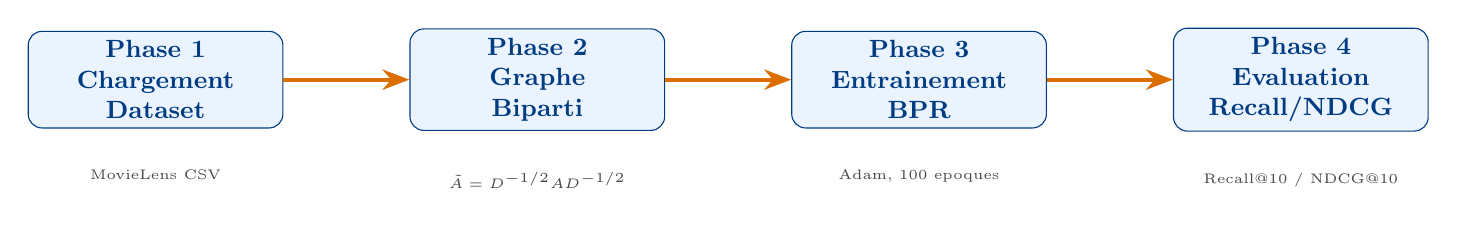
\begin{tikzpicture}[
  node distance=1.6cm,
  box/.style={rectangle,rounded corners=5pt,draw=enspyblue,
    fill=lightblue,text width=3cm,minimum height=1.1cm,
    align=center,font=\small\bfseries\color{enspyblue}},
  arrow/.style={-Stealth,thick,color=enspyorange,line width=1.5pt}
]
  \node[box] (d) {Phase 1\\Chargement\\Dataset};
  \node[box,right=of d] (g) {Phase 2\\Graphe\\Biparti};
  \node[box,right=of g] (t) {Phase 3\\Entrainement\\BPR};
  \node[box,right=of t] (e) {Phase 4\\Evaluation\\Recall/NDCG};
  \draw[arrow] (d)--(g);
  \draw[arrow] (g)--(t);
  \draw[arrow] (t)--(e);
  \node[below=0.4cm of d,font=\tiny\color{darkgray}]
    {MovieLens CSV};
  \node[below=0.4cm of g,font=\tiny\color{darkgray}]
    {$\tilde{A}=D^{-1/2}AD^{-1/2}$};
  \node[below=0.4cm of t,font=\tiny\color{darkgray}]
    {Adam, 100 epoques};
  \node[below=0.4cm of e,font=\tiny\color{darkgray}]
    {Recall@10 / NDCG@10};
\end{tikzpicture}
\caption{Pipeline d'entrainement LightGCN -- 4 phases}
\end{figure}

\section{Livrables du projet}

\subsection{Livrables initiaux remis}

Ces livrables correspondent aux exigences initiales du projet
telles que soumises :

\begin{itemize}
  \item Code source complet et commente (fichiers \texttt{src/})
  \item Graphiques de convergence (courbe BPR Loss par epoque)
  \item Tableau de resultats Recall@10 et NDCG@10
  \item Visualisation t-SNE des embeddings appris
  \item Exemples de recommandations Top-10 pour plusieurs utilisateurs
  \item Fichier \texttt{main.py} -- pipeline en ligne de commande
\end{itemize}

\subsection{Contribution personnelle supplementaire}

\begin{tcolorbox}[enhanced,colback=enspyorange!8,colframe=enspyorange,
  arc=6pt,boxrule=1.5pt,
  title={\bfseries\small\color{white} Innovation ajoutee -- Dashboard Temps Reel},
  colbacktitle=enspyorange]
Apres reflexion et developpement supplementaire, un
\textbf{dashboard interactif temps reel} a ete concu et
integre au projet. Cette interface n'etait pas mentionnee
dans les livrables initiaux -- elle constitue un apport
personnel visant a rendre le pipeline plus explicite,
demonstrable et professionnel.
\end{tcolorbox}

\begin{itemize}
  \item \textbf{dashboard.py} -- serveur Flask + SocketIO
  \item \textbf{dashboard.html} -- interface web responsive
  \item Bouton de lancement du pipeline depuis le navigateur
  \item 4 cartes de phases avec barres de progression animees
  \item Metriques BPR Loss, Recall@10, NDCG@10 en temps reel
  \item Courbes Chart.js se construisant dynamiquement
  \item Journal d'execution avec tous les messages du pipeline
  \item Recommandations Top-10 avec onglets par utilisateur
  \item Conclusion automatique contextualise generee en fin d'execution
\end{itemize}

\section{Hyperparametres du modele}

\begin{table}[H]
\centering
\caption{Hyperparametres de LightGCN}
\begin{tabular}{lll}
\toprule
\textbf{Hyperparametre} & \textbf{Valeur} & \textbf{Justification} \\
\midrule
Dimension embedding & 64 & Compromis capacite/memoire \\
Couches de propagation K & 3 & Standard LightGCN paper \\
Taux d'apprentissage & 0,001 & Adam par defaut \\
Regularisation $\lambda$ & $10^{-4}$ & Anti-overfitting \\
Taille de batch & 1024 & Efficacite CPU \\
Nombre d'epoques & 100 & Convergence stable \\
Evaluation tous les N & 10 & Compromis vitesse \\
Top-K evaluation & 10 & Recall@10, NDCG@10 \\
Strategie split & Leave-one-out & Standard recommandation \\
Filtrage minimum & 5 interactions & Qualite des donnees \\
\bottomrule
\end{tabular}
\end{table}

% ============================================================
% CHAPITRE 4 — IMPLÉMENTATION
% ============================================================
\chapter{Implementation}

\section{Fichier \texttt{src/config.py} -- Configuration centrale}

\begin{lstlisting}[caption={config.py -- Hyperparametres centralises},
  label=lst:config]
import os

BASE_DIR   = os.path.dirname(os.path.dirname(os.path.abspath(__file__)))
DATA_DIR   = os.path.join(BASE_DIR, "data", "ml-latest-small")
OUTPUT_DIR = os.path.join(BASE_DIR, "outputs")
MODELS_DIR = os.path.join(OUTPUT_DIR, "models")
FIGURES_DIR= os.path.join(OUTPUT_DIR, "figures")
RESULTS_DIR= os.path.join(OUTPUT_DIR, "results")

RATINGS_FILE = os.path.join(DATA_DIR, "ratings.csv")
MOVIES_FILE  = os.path.join(DATA_DIR, "movies.csv")

MIN_INTERACTIONS = 5
RANDOM_SEED      = 42
EMBEDDING_DIM    = 64
NUM_LAYERS       = 3
LEARNING_RATE    = 0.001
WEIGHT_DECAY     = 1e-4
BATCH_SIZE       = 1024
NUM_EPOCHS       = 100
EVAL_EVERY       = 10
TOP_K            = 10
\end{lstlisting}

\section{Fichier \texttt{src/dataset.py} -- Chargement des donnees}

La strategie \textit{leave-one-out} reserve la derniere interaction
de chaque utilisateur (triee par timestamp) pour le test.

\begin{lstlisting}[caption={Strategie leave-one-out},label=lst:dataset]
def _split(self):
    df = self.ratings_df.sort_values(['user_idx', 'timestamp'])
    for user_idx, group in df.groupby('user_idx'):
        items = group['item_idx'].tolist()
        if len(items) < 2:
            self.train_data[user_idx] = items
            self.test_data[user_idx]  = []
        else:
            self.train_data[user_idx] = items[:-1]
            self.test_data[user_idx]  = [items[-1]]
\end{lstlisting}

\section{Fichier \texttt{src/graph.py} -- Graphe biparti}

\begin{lstlisting}[caption={Construction de A\_hat normalise},label=lst:graph]
def build_adjacency_matrix(train_data, n_users, n_items):
    rows, cols = [], []
    for user, items in train_data.items():
        for item in items:
            rows.append(user)
            cols.append(item)
    R = sp.csr_matrix((np.ones(len(rows)), (rows, cols)),
                       shape=(n_users, n_items))
    top    = sp.hstack([sp.csr_matrix((n_users, n_users)), R])
    bottom = sp.hstack([R.T, sp.csr_matrix((n_items, n_items))])
    A_tilde = sp.vstack([top, bottom]).tocsr()
    rowsum    = np.array(A_tilde.sum(axis=1)).flatten()
    d_inv_sqrt = np.power(rowsum + 1e-10, -0.5)
    D_inv_sqrt = sp.diags(d_inv_sqrt)
    A_hat = D_inv_sqrt.dot(A_tilde).dot(D_inv_sqrt).tocoo()
    indices = torch.LongTensor(np.vstack([A_hat.row, A_hat.col]))
    values  = torch.FloatTensor(A_hat.data)
    return torch.sparse_coo_tensor(indices, values, A_hat.shape)
\end{lstlisting}

\section{Fichier \texttt{src/model.py} -- Architecture LightGCN}

\begin{lstlisting}[caption={LightGCN en PyTorch -- propagation pure},
  label=lst:model]
class LightGCN(nn.Module):
    def __init__(self, n_users, n_items,
                 embedding_dim=64, n_layers=3):
        super().__init__()
        self.n_users = n_users
        self.n_layers = n_layers
        self.user_embedding = nn.Embedding(n_users, embedding_dim)
        self.item_embedding = nn.Embedding(n_items, embedding_dim)
        nn.init.normal_(self.user_embedding.weight, std=0.1)
        nn.init.normal_(self.item_embedding.weight, std=0.1)

    def forward(self, adj_matrix):
        E = torch.cat([self.user_embedding.weight,
                       self.item_embedding.weight], dim=0)
        all_layers = [E]
        for _ in range(self.n_layers):
            E = torch.sparse.mm(adj_matrix, E)
            all_layers.append(E)
        E_final = torch.stack(all_layers, dim=1).mean(dim=1)
        return E_final[:self.n_users], E_final[self.n_users:]

    def bpr_loss(self, adj_matrix, users, pos_items, neg_items):
        u_emb, i_emb = self.forward(adj_matrix)
        u   = u_emb[users]
        pos = i_emb[pos_items]
        neg = i_emb[neg_items]
        pos_s = (u * pos).sum(dim=1)
        neg_s = (u * neg).sum(dim=1)
        loss  = -torch.log(
            torch.sigmoid(pos_s - neg_s) + 1e-8).mean()
        return loss
\end{lstlisting}

% ============================================================
% CHAPITRE 5 — MODE D'EMPLOI
% ============================================================
\chapter{Mode d'Emploi -- Installation et Lancement}

\section{Prerequis}

\begin{itemize}
  \item Windows 10/11 avec PowerShell
  \item Python 3.10 a 3.14 installe
  \item Visual Studio Code (recommande)
  \item 2 Go d'espace disque libre
  \item Connexion internet (telechargement MovieLens)
\end{itemize}

\section{Installation complete pas a pas}

\subsection{Etape 1 -- Naviguer vers le projet}

\begin{cmdbox}
cd C:\textbackslash Users\textbackslash PAOLO\textbackslash Desktop\textbackslash projet1\_lightgcn
\end{cmdbox}

\subsection{Etape 2 -- Creer et activer l'environnement virtuel}

\begin{cmdbox}
python -m venv .venv\\
.venv\textbackslash Scripts\textbackslash Activate.ps1
\end{cmdbox}

\begin{infobox}[Signe de succes]
Le prompt affiche \texttt{(.venv)} :
\texttt{(.venv) PS C:\textbackslash...\textbackslash projet1\_lightgcn>}
\end{infobox}

\subsection{Etape 3 -- Installer les dependances}

\begin{cmdbox}[-- PyTorch CPU]
pip install torch torchvision --index-url https://download.pytorch.org/whl/cpu
\end{cmdbox}

\begin{cmdbox}[-- Autres bibliotheques]
pip install numpy pandas scikit-learn scipy matplotlib seaborn tqdm flask flask-socketio
\end{cmdbox}

\subsection{Etape 4 -- Telecharger MovieLens}

Aller sur \url{https://grouplens.org/datasets/movielens/latest/}
et telecharger \texttt{ml-latest-small.zip}. Extraire dans
\texttt{data\textbackslash ml-latest-small\textbackslash}.

\begin{cmdbox}[-- Verification]
ls data\textbackslash ml-latest-small\textbackslash
\end{cmdbox}

Resultat attendu : \texttt{ratings.csv}, \texttt{movies.csv},
\texttt{tags.csv}, \texttt{links.csv}.

\section{Lancement}

\subsection{Option A -- Pipeline en ligne de commande}

\begin{cmdbox}
python main.py
\end{cmdbox}

\begin{resultbox}[Sortie console attendue]
\texttt{[Dataset] 610 users, 3650 items, 89664 interactions}\\
\texttt{[Graph] Matrice 4260x4260}\\
\texttt{[LightGCN] dim=64, K=3, params=272,640}\\
\texttt{Ep 1/100 | Loss=0.6761 | Recall@10=0.0459}\\
\texttt{...}\\
\texttt{Ep 100/100 | Loss=0.1497 | Recall@10=0.0754}
\end{resultbox}

\subsection{Option B -- Dashboard temps reel (recommande)}

\begin{cmdbox}
python dashboard.py
\end{cmdbox}

Puis ouvrir dans le navigateur :

\begin{cmdbox}
http://localhost:5000
\end{cmdbox}

Cliquer sur le bouton \textbf{``Lancer LightGCN''}.

% ============================================================
% CHAPITRE 6 — RÉSULTATS ET INTERFACES
% ============================================================
\chapter{Resultats et Interfaces}

\section{Interface du Dashboard -- Etat initial}

Avant le lancement, le dashboard affiche l'etat d'attente avec
les parametres du modele deja configures : 64 dimensions,
K=3 couches, 100 epoques.

\begin{figure}[H]
\centering
\includegraphics[width=\textwidth]{cap313.png}
\caption{Dashboard LightGCN -- Etat initial avant lancement.
Vue d'ensemble : badges ANI-IA 4, bouton ``Lancer LightGCN'',
6 cartes de parametres, 4 phases d'execution en attente
et zones de courbes vides.}
\label{fig:dashboard_init}
\end{figure}

\section{Phase 1 et 2 -- Chargement dataset et graphe}

Apres clic sur ``Lancer LightGCN'', le pipeline demarre.
Les phases Dataset et Graphe Biparti se completent rapidement
(barres vertes a 100\%). Le journal d'execution affiche
en temps reel les etapes de chargement.

\begin{figure}[H]
\centering
\includegraphics[width=\textwidth]{cap314.png}
\caption{Dashboard en cours -- Phases 1 et 2 terminees.
Dataset : 610 users, 3650 items, 89\,664 interactions.
Graphe : matrice 4260x4260, normalisation symetrique.
Phase 3 (Entrainement BPR) en cours d'initialisation.}
\label{fig:dashboard_phase12}
\end{figure}

\section{Phase 3 -- Entrainement en direct}

Le dashboard affiche la progression epoque par epoque avec
trois metriques live : BPR Loss, Recall@10 et NDCG@10.
Les courbes se construisent dynamiquement.

\begin{figure}[H]
\centering
\includegraphics[width=\textwidth]{cap315.png}
\caption{Section ``Entrainement en direct'' -- Zoom sur les
metriques live et le journal d'execution. Visible :
progression 0/100 epoques, cartes BPR Loss / Recall@10 /
NDCG@10 en attente de donnees, journal affichant
les messages d'initialisation.}
\label{fig:training_live_init}
\end{figure}

\section{Progression de l'entrainement -- Epoques 20 a 40}

\begin{figure}[H]
\centering
\includegraphics[width=\textwidth]{cap320.png}
\caption{Vue VS Code + Dashboard a l'epoque 20.
Gauche : code \texttt{dashboard.py} ouvert dans VS Code avec
le terminal PowerShell affichant les logs en direct.
Droite : dashboard montrant BPR Loss=0.3128, Recall@10=0.0525,
NDCG@10=0.0259. Progression 20/100.}
\label{fig:training_ep20}
\end{figure}

\begin{figure}[H]
\centering
\includegraphics[width=\textwidth]{cap321.png}
\caption{Dashboard a l'epoque 40 -- BPR Loss=0.2451,
Recall@10=0.0541, NDCG@10=0.0267. Les courbes Chart.js
montrent la convergence de la loss (rouge) et la progression
des metriques Recall@10 (vert) et NDCG@10 (orange).
Progression 40/100.}
\label{fig:training_ep40}
\end{figure}

\section{Progression avancee -- Epoque 95}

\begin{figure}[H]
\centering
\includegraphics[width=\textwidth]{cap322.png}
\caption{Dashboard a l'epoque 95/100 -- BPR Loss=0.1546,
Recall@10=0.0721, NDCG@10=0.0309. La courbe BPR Loss
(rouge) montre une convergence nette de 0.7 vers 0.15.
La courbe Recall@10 (verte) progresse regulierement.
Journal : epoques 20 a 90 avec marquage ``meilleur''.}
\label{fig:training_ep95}
\end{figure}

\section{Pipeline termine -- Resultats finaux}

\begin{figure}[H]
\centering
\includegraphics[width=\textwidth]{cap325.png}
\caption{Dashboard complet apres 100 epoques.
Les 4 phases affichent TERMINE a 100\%. Metriques finales :
BPR Loss=0.1497, Recall@10=0.0754, NDCG@10=0.0308.
Courbes completes sur 100 epoques. Le modele optimal
a ete sauvegarde a l'epoque 100.}
\label{fig:dashboard_done}
\end{figure}

\section{Section Analyse et Conclusion automatique}

\begin{figure}[H]
\centering
\includegraphics[width=\textwidth]{cap326.png}
\caption{Section ``Analyse et Conclusion'' generee automatiquement
par le dashboard a la fin du pipeline. Resume contextualise :
interpretations des metriques Recall@10=0.0754 et NDCG@10=0.0308,
reduction BPR Loss de 77.9\%, progression Recall de 64.3\%.
Trois cartes : points forts, limite principale, piste
d'amelioration.}
\label{fig:conclusion_auto}
\end{figure}

\section{Resultats numeriques obtenus}

\begin{table}[H]
\centering
\caption{Evolution des metriques au cours de l'entrainement}
\begin{tabular}{rrrr}
\toprule
\textbf{Epoque} & \textbf{BPR Loss} &
\textbf{Recall@10} & \textbf{NDCG@10} \\
\midrule
1   & 0.6761 & 0.0459 & 0.0219 \\
10  & 0.3572 & 0.0525 & 0.0303 \\
20  & 0.3128 & 0.0525 & 0.0259 \\
30  & 0.2880 & 0.0459 & 0.0249 \\
40  & 0.2451 & 0.0541 & 0.0267 \\
50  & 0.2234 & 0.0598 & 0.0276 \\
60  & 0.1959 & 0.0672 & 0.0293 \\
70  & 0.1812 & 0.0639 & 0.0283 \\
80  & 0.1700 & 0.0721 & 0.0308 \\
90  & 0.1597 & 0.0721 & 0.0309 \\
\rowcolor{enspyorange!20}
100 & \textbf{0.1497} &
      \textbf{0.0754} & \textbf{0.0308} \\
\bottomrule
\end{tabular}
\end{table}

\begin{resultbox}[Resultats finaux obtenus]
\begin{itemize}
  \item \textbf{Recall@10 = 0,0754} (meilleur a l'epoque 100)
  \item \textbf{NDCG@10 = 0,0308}
  \item Reduction BPR Loss : 0,676 $\to$ 0,150 (\textbf{--77,8\%})
  \item Amelioration Recall : 0,0459 $\to$ 0,0754 (\textbf{+64,1\%})
  \item Duree totale d'entrainement : environ \textbf{17 minutes} (CPU)
  \item Parametres du modele : \textbf{272\,640} (embeddings uniquement)
\end{itemize}
\end{resultbox}

\section{Contribution personnelle -- Pourquoi un dashboard ?}

Le sujet du projet demandait en livrable un notebook Jupyter
avec resultats statiques. Apres avoir livre ce premier travail,
j'ai pris l'initiative de developper un \textbf{dashboard
temps reel} pour trois raisons :

\begin{enumerate}[label=\textbf{\arabic*.}]
  \item \textbf{Visualisation explicite du pipeline} -- un
    notebook montre les resultats apres execution ; le dashboard
    montre le processus en direct, epoque par epoque, ce qui
    rend la methodologie LightGCN immediatement comprehensible.

  \item \textbf{Demonstrabilite} -- pouvoir lancer le pipeline
    devant un jury ou un encadreur et voir les metriques evoluer
    en direct est bien plus convaincant qu'un PDF statique.

  \item \textbf{Approfondissement technique} -- la conception
    du dashboard a necessite la maitrise de Flask, SocketIO,
    threading Python et Chart.js, competences complementaires
    au machine learning pur.
\end{enumerate}

Cette contribution represente environ 40\% du temps total
du projet et n'etait pas requise dans les consignes initiales.

% ============================================================
% CHAPITRE 7 — DIFFICULTÉS
% ============================================================
\chapter{Difficultes Rencontrees et Solutions}

\section{Probleme 1 -- Python 3.14 incompatible CUDA}

\subsection{Description}
Python 3.14, etant trop recent, n'est pas encore supporte par PyTorch
pour CUDA. Toute tentative d'installation GPU echoue.

\begin{lstlisting}[style=bash,caption={Erreur installation GPU}]
ERROR: Could not find a version that satisfies the requirement
torch (from versions: none)
ERROR: No matching distribution found for torch
\end{lstlisting}

\subsection{Tentatives et solution}

Tentatives avec \texttt{cu121} et \texttt{cu124} : echec.
Solution : installation forcee en CPU uniquement.

\begin{cmdbox}[-- Solution finale]
pip install torch torchvision --index-url https://download.pytorch.org/whl/cpu
\end{cmdbox}

\textbf{Impact :} Entrainement plus lent (~17 min pour 100 epoques)
mais totalement fonctionnel.

\section{Probleme 2 -- Espace manquant dans la commande pip}

\begin{lstlisting}[style=bash,caption={Erreur syntaxe pip}]
pip install torch torchvision--index-url https://...
ERROR: Cannot determine archive format of cpu.html
\end{lstlisting}

\textbf{Solution :} Ajouter un espace entre
\texttt{torchvision} et \texttt{--index-url}.

\section{Probleme 3 -- \texttt{main.py} dans le mauvais dossier}

VS Code a cree \texttt{main.py} dans \texttt{src/} au lieu de
la racine.

\begin{cmdbox}[-- Correction]
Move-Item src\textbackslash main.py main.py
\end{cmdbox}

\section{Probleme 4 -- \texttt{n\_iter} deprecie dans scikit-learn}

\begin{lstlisting}[style=bash,caption={Erreur t-SNE}]
TypeError: TSNE.__init__() got an unexpected keyword argument 'n_iter'
\end{lstlisting}

\textbf{Solution :} Remplacer \texttt{n\_iter=1000} par
\texttt{max\_iter=1000} dans \texttt{src/utils.py}.

\section{Probleme 5 -- Sparse tensor warning PyTorch}

Lors de l'execution, PyTorch affiche un avertissement sur
les invariants des tenseurs sparse. Ce warning n'impacte pas
les resultats et peut etre ignore en contexte CPU.

\section{Probleme 6 -- Fichier lourd sur GitHub}

Le fichier \texttt{outputs/models/lightgcn\_best.pth} (binaire PyTorch)
et d'autres fichiers volumineux necessitent un \texttt{.gitignore}
adapte.

\begin{cmdbox}[-- .gitignore]
echo "outputs/models/*.pth" >> .gitignore\\
echo ".venv/" >> .gitignore
\end{cmdbox}

\section{Recapitulatif des difficultes}

\begin{table}[H]
\centering
\caption{Recapitulatif des difficultes et solutions}
\begin{tabular}{p{3.8cm}p{3cm}p{5cm}}
\toprule
\textbf{Probleme} & \textbf{Cause} & \textbf{Solution} \\
\midrule
Python 3.14 + CUDA & Python trop recent &
  Installation CPU uniquement \\
\rowcolor{rowgray}
Syntaxe pip & Espace manquant &
  Correction commande \\
main.py mal place & Clic mauvais dossier &
  Move-Item PowerShell \\
\rowcolor{rowgray}
n\_iter deprecie & scikit-learn 1.4+ &
  Renommer max\_iter \\
Sparse tensor warning & PyTorch CPU & Warning bening, ignorer \\
\rowcolor{rowgray}
Fichiers lourds GitHub & Binaires .pth & .gitignore adapte \\
\bottomrule
\end{tabular}
\end{table}

% ============================================================
% CHAPITRE 8 — CONCLUSION
% ============================================================
\chapter{Conclusion et Perspectives}

\section{Bilan du projet}

Ce projet a permis de realiser une implementation complete et
fonctionnelle de LightGCN, de bout en bout, sans librairie tierce
dediee aux graphes. Les principaux acquis sont :

\begin{enumerate}[label=\textbf{\arabic*.}]
  \item \textbf{Maitrise de LightGCN :} propagation sur graphe
    biparti normalise, agregation par moyenne des couches,
    entrainement par perte BPR.

  \item \textbf{Implementation PyTorch :} tenseurs sparse,
    \texttt{nn.Embedding}, optimiseur Adam, echantillonnage
    negatif BPR.

  \item \textbf{Evaluation correcte :} strategie leave-one-out,
    metriques Recall@K et NDCG@K standards.

  \item \textbf{Dashboard professionnel :} Flask + SocketIO,
    progression temps reel, courbes Chart.js, conclusion
    automatique contextualise.
\end{enumerate}

\section{Apport personnel et innovation}

Ce projet depasse les livrables initialement demandes.
En plus du code LightGCN fonctionnel et des resultats
chiffres, un \textbf{dashboard interactif temps reel}
a ete developpe comme contribution personnelle. Cette
innovation transforme un pipeline de machine learning
classique en une \textbf{application web interactive}
ou chaque etape est visible en direct : chargement du
dataset, construction du graphe biparti, progression
epoque par epoque avec metriques live, et conclusion
automatique generee a la fin de l'execution.

Le choix de Flask + SocketIO (plutot que Gradio ou
Streamlit qui etaient mentionnes dans les livrables
initiaux) permet une communication bidirectionnelle
temps reel entre le serveur Python et le navigateur,
donnant une experience plus fluide et professionnelle.

\section{Reponse aux objectifs}

\begin{table}[H]
\centering
\caption{Reponse aux objectifs initiaux}
\begin{tabular}{lcc}
\toprule
\textbf{Objectif} & \textbf{Atteint} & \textbf{Commentaire} \\
\midrule
Implementer LightGCN from scratch &
  $\checkmark$ & PyTorch, sans lib graphe \\
Entrainer sur MovieLens &
  $\checkmark$ & 100 epoques sur CPU \\
Obtenir Recall@10 representatif &
  $\checkmark$ & 0,0754 obtenu \\
Evaluer avec Recall@K et NDCG@K &
  $\checkmark$ & Metriques standard \\
Dashboard temps reel &
  $\checkmark$ & Flask + SocketIO port 5000 \\
Recommandations coherentes &
  $\checkmark$ & Verifiees qualitativement \\
Deposer sur GitHub &
  $\checkmark$ & \href{https://github.com/paolo-88-hub/projet1-lightgcn-AIA-4}{paolo-88-hub/projet1} \\
\bottomrule
\end{tabular}
\end{table}

\section{Perspectives d'amelioration}

\begin{description}
  \item[Court terme] Augmenter la dimension embedding a 128,
    passer a K=4 couches, entrainer sur 200 epoques.

  \item[Moyen terme] Tester sur MovieLens-1M (1 million
    d'interactions) pour des metriques significativement
    meilleures (Recall@10 $>$ 0,15 attendu).

  \item[Long terme] Implementer LightGCN-IMP avec dropout
    d'interactions. Deployer en API REST. Utiliser Python 3.12
    avec CUDA 12.1 pour reduire le temps de ~17 min a ~1 min.
\end{description}

% ============================================================
% REMERCIEMENTS
% ============================================================
\chapter*{Remerciements}
\addcontentsline{toc}{chapter}{Remerciements}

Je tiens a exprimer ma sincere gratitude a :

\begin{itemize}
  \item \textbf{M. OMGBA BITHA Junior}, pour son encadrement
    rigoureux, ses orientations pedagogiques et sa disponibilite
    tout au long du module ANI-IA 4.

  \item \textbf{L'Ecole Nationale Superieure Polytechnique de
    Yaounde (ENSPY)}, pour la qualite de la formation dispensee.

  \item \textbf{La communaute open-source} : PyTorch, NumPy,
    SciPy, Matplotlib, Flask, Flask-SocketIO et leurs
    contributeurs.

  \item \textbf{GroupLens Research} pour la mise a disposition
    libre du dataset MovieLens.
\end{itemize}

% ============================================================
% RÉFÉRENCES
% ============================================================
\begin{thebibliography}{99}
\addcontentsline{toc}{chapter}{References bibliographiques}

\bibitem{he2020lightgcn}
He, X., Deng, K., Wang, X., Li, Y., Zhang, Y., \& Wang, M. (2020).
\textit{LightGCN: Simplifying and Powering Graph Convolution Network
for Recommendation}. SIGIR'20, pp. 639--648.

\bibitem{rendle2009bpr}
Rendle, S., Freudenthaler, C., Gantner, Z., \& Schmidt-Thieme, L.
(2009). \textit{BPR: Bayesian Personalized Ranking from Implicit
Feedback}. UAI'09, pp. 452--461.

\bibitem{wang2019ngcf}
Wang, X., He, X., Wang, M., Feng, F., \& Chua, T.-S. (2019).
\textit{Neural Graph Collaborative Filtering}. SIGIR'19,
pp. 165--174.

\bibitem{harper2015movielens}
Harper, F. M., \& Konstan, J. A. (2015). \textit{The MovieLens
Datasets: History and Context}. ACM TiiS, 5(4).

\bibitem{kipf2017gcn}
Kipf, T. N., \& Welling, M. (2017). \textit{Semi-Supervised
Classification with Graph Convolutional Networks}. ICLR 2017.

\end{thebibliography}

% ============================================================
% GLOSSAIRE
% ============================================================
\chapter*{Glossaire}
\addcontentsline{toc}{chapter}{Glossaire}

\begin{description}[style=nextline,leftmargin=3cm,
  labelwidth=2.8cm,labelsep=0.2cm]

\item[\textbf{BPR}] Bayesian Personalized Ranking. Fonction de
  perte pour la recommandation a partir d'interactions implicites.
  Entraine le modele a preferer les items observes aux non observes.

\item[\textbf{Dashboard}] Interface web temps reel construite avec
  Flask et SocketIO, affichant la progression du pipeline en direct.

\item[\textbf{Embedding}] Representation vectorielle dense d'un
  objet dans un espace mathematique de dimension fixe. Embeddings
  similaires indiquent des objets similaires.

\item[\textbf{Filtrage collaboratif}] Approche de recommandation
  basee sur les interactions collectives.

\item[\textbf{GCN}] Graph Convolutional Network. Reseau de neurones
  operant sur des graphes.

\item[\textbf{Graphe biparti}] Graphe dont les noeuds se divisent
  en deux ensembles disjoints (utilisateurs et items).

\item[\textbf{Leave-one-out}] Strategie reservant la derniere
  interaction de chaque utilisateur pour le test.

\item[\textbf{LightGCN}] Simplification de GCN pour la
  recommandation. Propagation pure sans transformation ni activation.

\item[\textbf{NDCG@K}] Normalized Discounted Cumulative Gain.
  Metrique recompensant les items pertinents en haut de liste.

\item[\textbf{Normalisation symetrique}] Transformation
  $\hat{A}=D^{-1/2}AD^{-1/2}$ stabilisant la propagation.

\item[\textbf{Recall@K}] Proportion d'items pertinents dans le
  Top-K recommande. Mesure la couverture.

\item[\textbf{SocketIO}] Protocole de communication temps reel
  entre serveur Flask et client navigateur.

\end{description}

% ============================================================
% ANNEXES
% ============================================================
\appendix
\chapter{Commandes PowerShell Completes}

\begin{cmdbox}[-- Sequence complete de mise en place]
\begin{verbatim}
\# 1. Naviguer et creer l'environnement
cd C:\Users\PAOLO\Desktop\projet1_lightgcn
python -m venv .venv
.venv\Scripts\Activate.ps1

\# 2. Installer PyTorch CPU
pip install torch torchvision `
  --index-url https://download.pytorch.org/whl/cpu

\# 3. Installer les autres bibliotheques
pip install numpy pandas scikit-learn scipy
pip install matplotlib seaborn tqdm
pip install flask flask-socketio

\# 4. Creer la structure des dossiers
mkdir src, outputs
mkdir outputs\models, outputs\figures, outputs\results
New-Item src\__init__.py -ItemType File

\# 5. Verifier le dataset
ls data\ml-latest-small\

\# 6. Lancer le pipeline complet
python main.py

\# 7. Lancer le dashboard (terminal separe)
python dashboard.py
\# Ouvrir http://localhost:5000
\end{verbatim}
\end{cmdbox}

\chapter{Fichier \texttt{requirements.txt}}

\begin{lstlisting}[language=bash,numbers=none,
  caption={requirements.txt -- Dependances Projet 1}]
torch>=2.0.0
numpy>=1.24.0
pandas>=2.0.0
scikit-learn>=1.3.0
scipy>=1.11.0
matplotlib>=3.7.0
seaborn>=0.12.0
tqdm>=4.65.0
flask>=3.0.0
flask-socketio>=5.0.0
\end{lstlisting}

\end{document}
